\section{Models}
With the question defined, the equations of motion derived, we can now consider the different models to achieve maximum displacement from a single jump.

% TODO: maybe put the constants before engine section
\subsection{Constants}
One might notice that I've deliberately left some of the constants $j_i$ clear of meaningful values and only suggested in-game default values. This is because many long-jumpers in the community find the default (vanilla) settings of the game engines ``bland'', reducing the excitement of this activity. Therefore, I will be setting some of the engine constants myself.

There are 4 of them:
\begin{itemize}
    \item \verb|sv_gravity| ($g$), set to 800
    \item \verb|sv_maxspeed| ($L$), set to 250
    \item \verb|sv_airaccelerate| ($A$), set to 10
    \item \verb|tickrate| ($n$), set to 64, or $\tau=\frac{1}{64}$
\end{itemize}

The only meaning deviation from the default settings are the speed limit $L$, for the default settings limits the optimization one can achieve, while the higher value of $250$ simply magnifies the result that one can achieve.

Furthermore, all models are free to set the initial velocity $\tv_0$, with the constraint that the magnitude of $\tv_0$ does not exceed $250$, the speed limit.

\subsection{Straight line}
% where you do nothing
We all know the fastest route (shortest distance) from point $A$ to point $B$ is with a straight line connecting $A$ to $B$. Therefore if the velocity magnitude is maximized, and as time is proportional to distance: $t = \frac{s}{\tmag{\tv}}$, it seems that a straight line would maximize the jumping distance assuming no constraints. This will serve as a good baseline for all the other models.

I have decided for the player to travel along the y-axis because I personally find it nicer to graph and draw with, but all maths would apply if you wish to substitute for the x-axis. This is represented by the acceleration function:

\begin{figure}[H]
    \centering
    \[
    \tunit{a}(t) = \tang{0, 1}
    \]
    \caption{The straight line model}
\end{figure}

Notice that player acceleration is constant in this model, and which can be achieved simply by looking forward, and press the key $w$ during the jump. Furthermore, we can set the initial velocity to point directly upwards in the y direction, such that:
\[
\tv_0 = \tang{0, 250},
\]
for common knowledge tells me that a faster initial speed in the direction where I am going will result in higher overall travel distance. Overall, there exists four metrics for each model, each worth evaluating.

We can first look at the case without the max speed constraint. By running a simulation with the engine constants discussed before, I got a result of $\approx 807.5$ hammer units in a jump. Predictably, this model will have the player traveling in a straight line (figure \ref{fig:straight_nothing_1}).

\begin{wrapfigure}{r}{0.48\textwidth}
    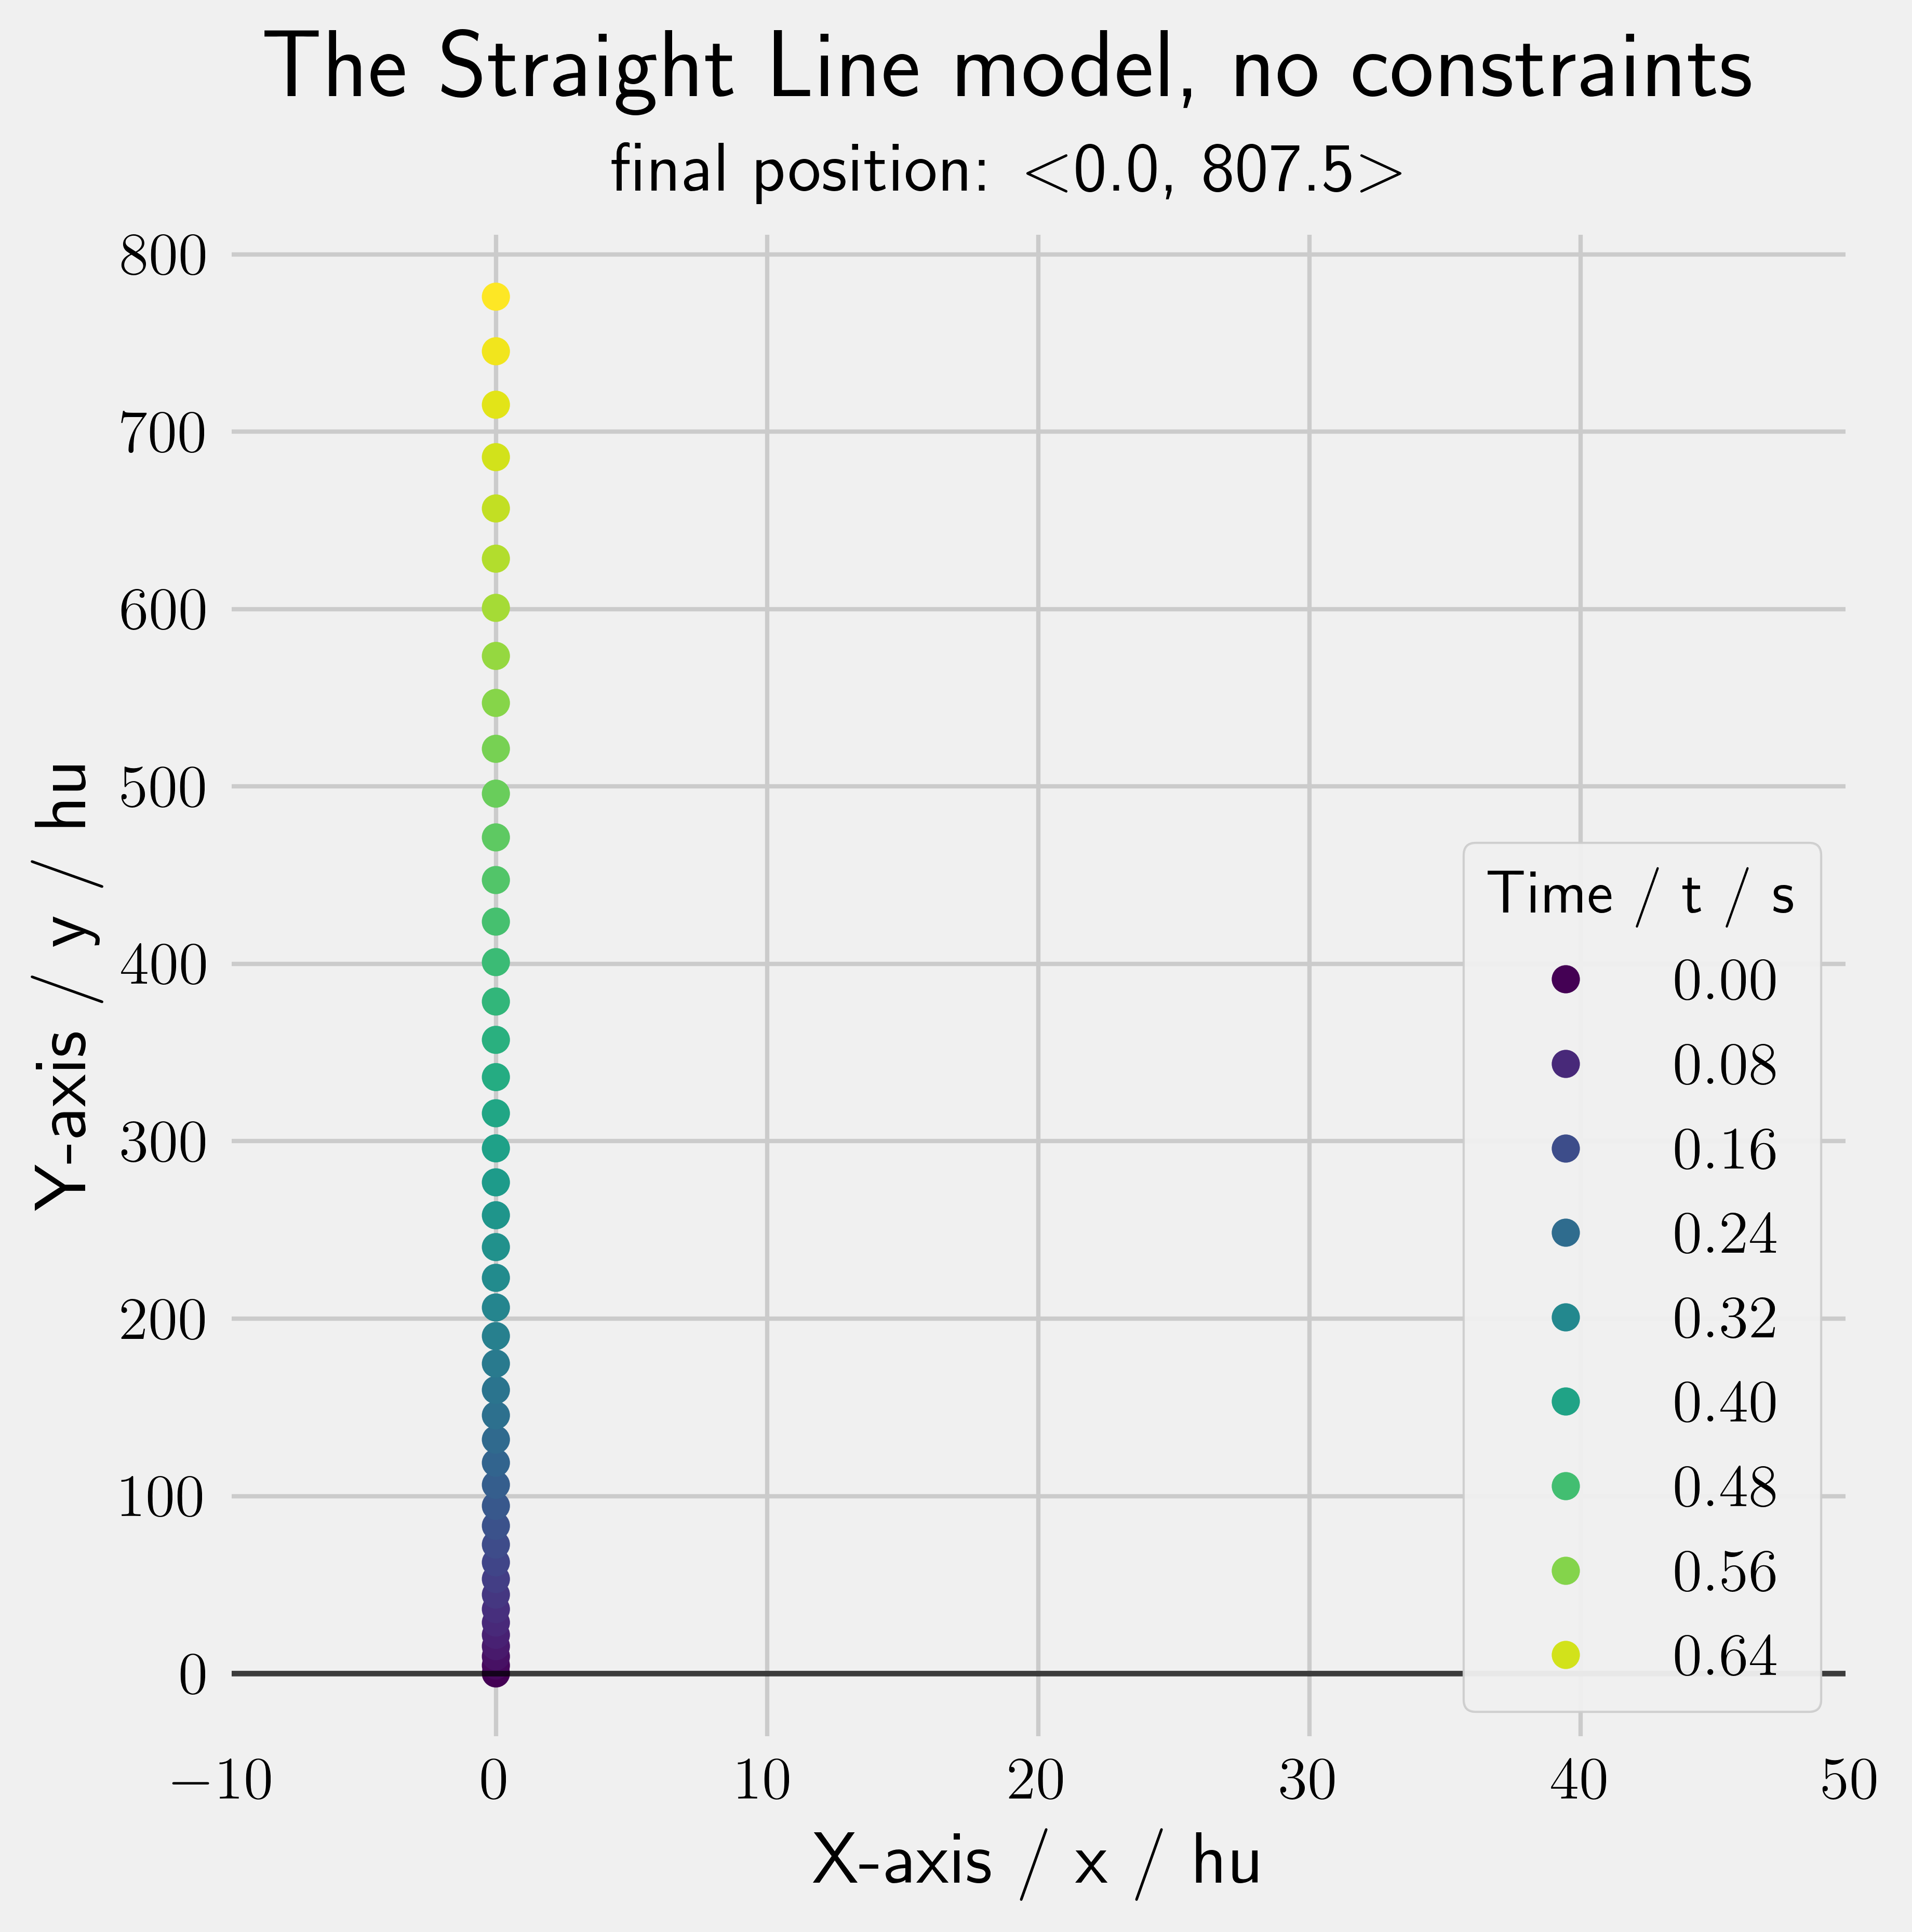
\includegraphics[width=0.45\textwidth,right]{assets/straight_nothing_1.png}
    \caption{}
    \label{fig:straight_nothing_1}
\end{wrapfigure}

I can comfortably say that this jumping distance would never be possible to achieve in game, for this model can be proven to be the most optimal jumping path if there are no speed limits (appendix, using EL equation). This number of around $800$ hammer units serves to be the upper-bound output of our optimization, and the lower-bound being its negative of around $-800$ (if you wish to accelerate directly backwards with negative initial velocity).

Additionally we can also utilize the equation derived in the last section (equations \ref{eq:jumping}).

Using the acceleration function, we can define $x(t)$ and $y(t)$ as:
\[
    x(t) = 0, \quad y(t) = 1.
\]

Their first and second order indefinite integrals can be obtained using calculus:
\begin{alignat*}{3}
    X(t) &= \int x(t) \, dx = 0, \quad
    &&\tfx(t) &&= \int X(t) \, dx = 0\\
    Y(t) &= \int y(t) \, dx = t, \quad
    &&\tfy(t) &&= \int Y(t) \, dx = \frac{1}{2} t^2,
\end{alignat*}
notice that the constants during integration are omitted as we've incorporated them into the derivation of the jumping motion equations as $c_1$, and $c_2$.

Therefore the $x$ position after $t_f$ seconds assuming no speed limit is:
\begin{align*}
    p_x &= p(t_f)_x = w\tfx(t_f) + t_f(v_{0x} - w\tfx'(0)) - w\tfx(0)\\
    &= w \times 0 + t_f(0 - w \times 0) - w \times 0\\
    &= 0,
\end{align*}
and the respective $y$ position is:
\begin{align*}
    p_y &= p(t_f)_y = w\tfy(t_f) + t_f(v_{0y} - w\tfy'(0)) - w\tfy(0)\\
    &= w \frac{1}{2} t_f^2 + t_f(v_{0y} - w v_{0y} \times 0) - w \times 0\\
    &= (10 \times 250) \frac{1}{2} (0.7)^2 + 0.7 \times 250\\
    &= 787.5
\end{align*}

% TODO: change A to 10

The jumping motion differential equations resulted in a similar sized jumping distance in comparison to the engine simulated $\approx807.5$. I believe that a $\frac{|787.5-807.5|}{807.5} \approx 2.48\%$ error is a very well approximation of this continuous method for future modeling.

\begin{wrapfigure}{r}{0.48\textwidth}
    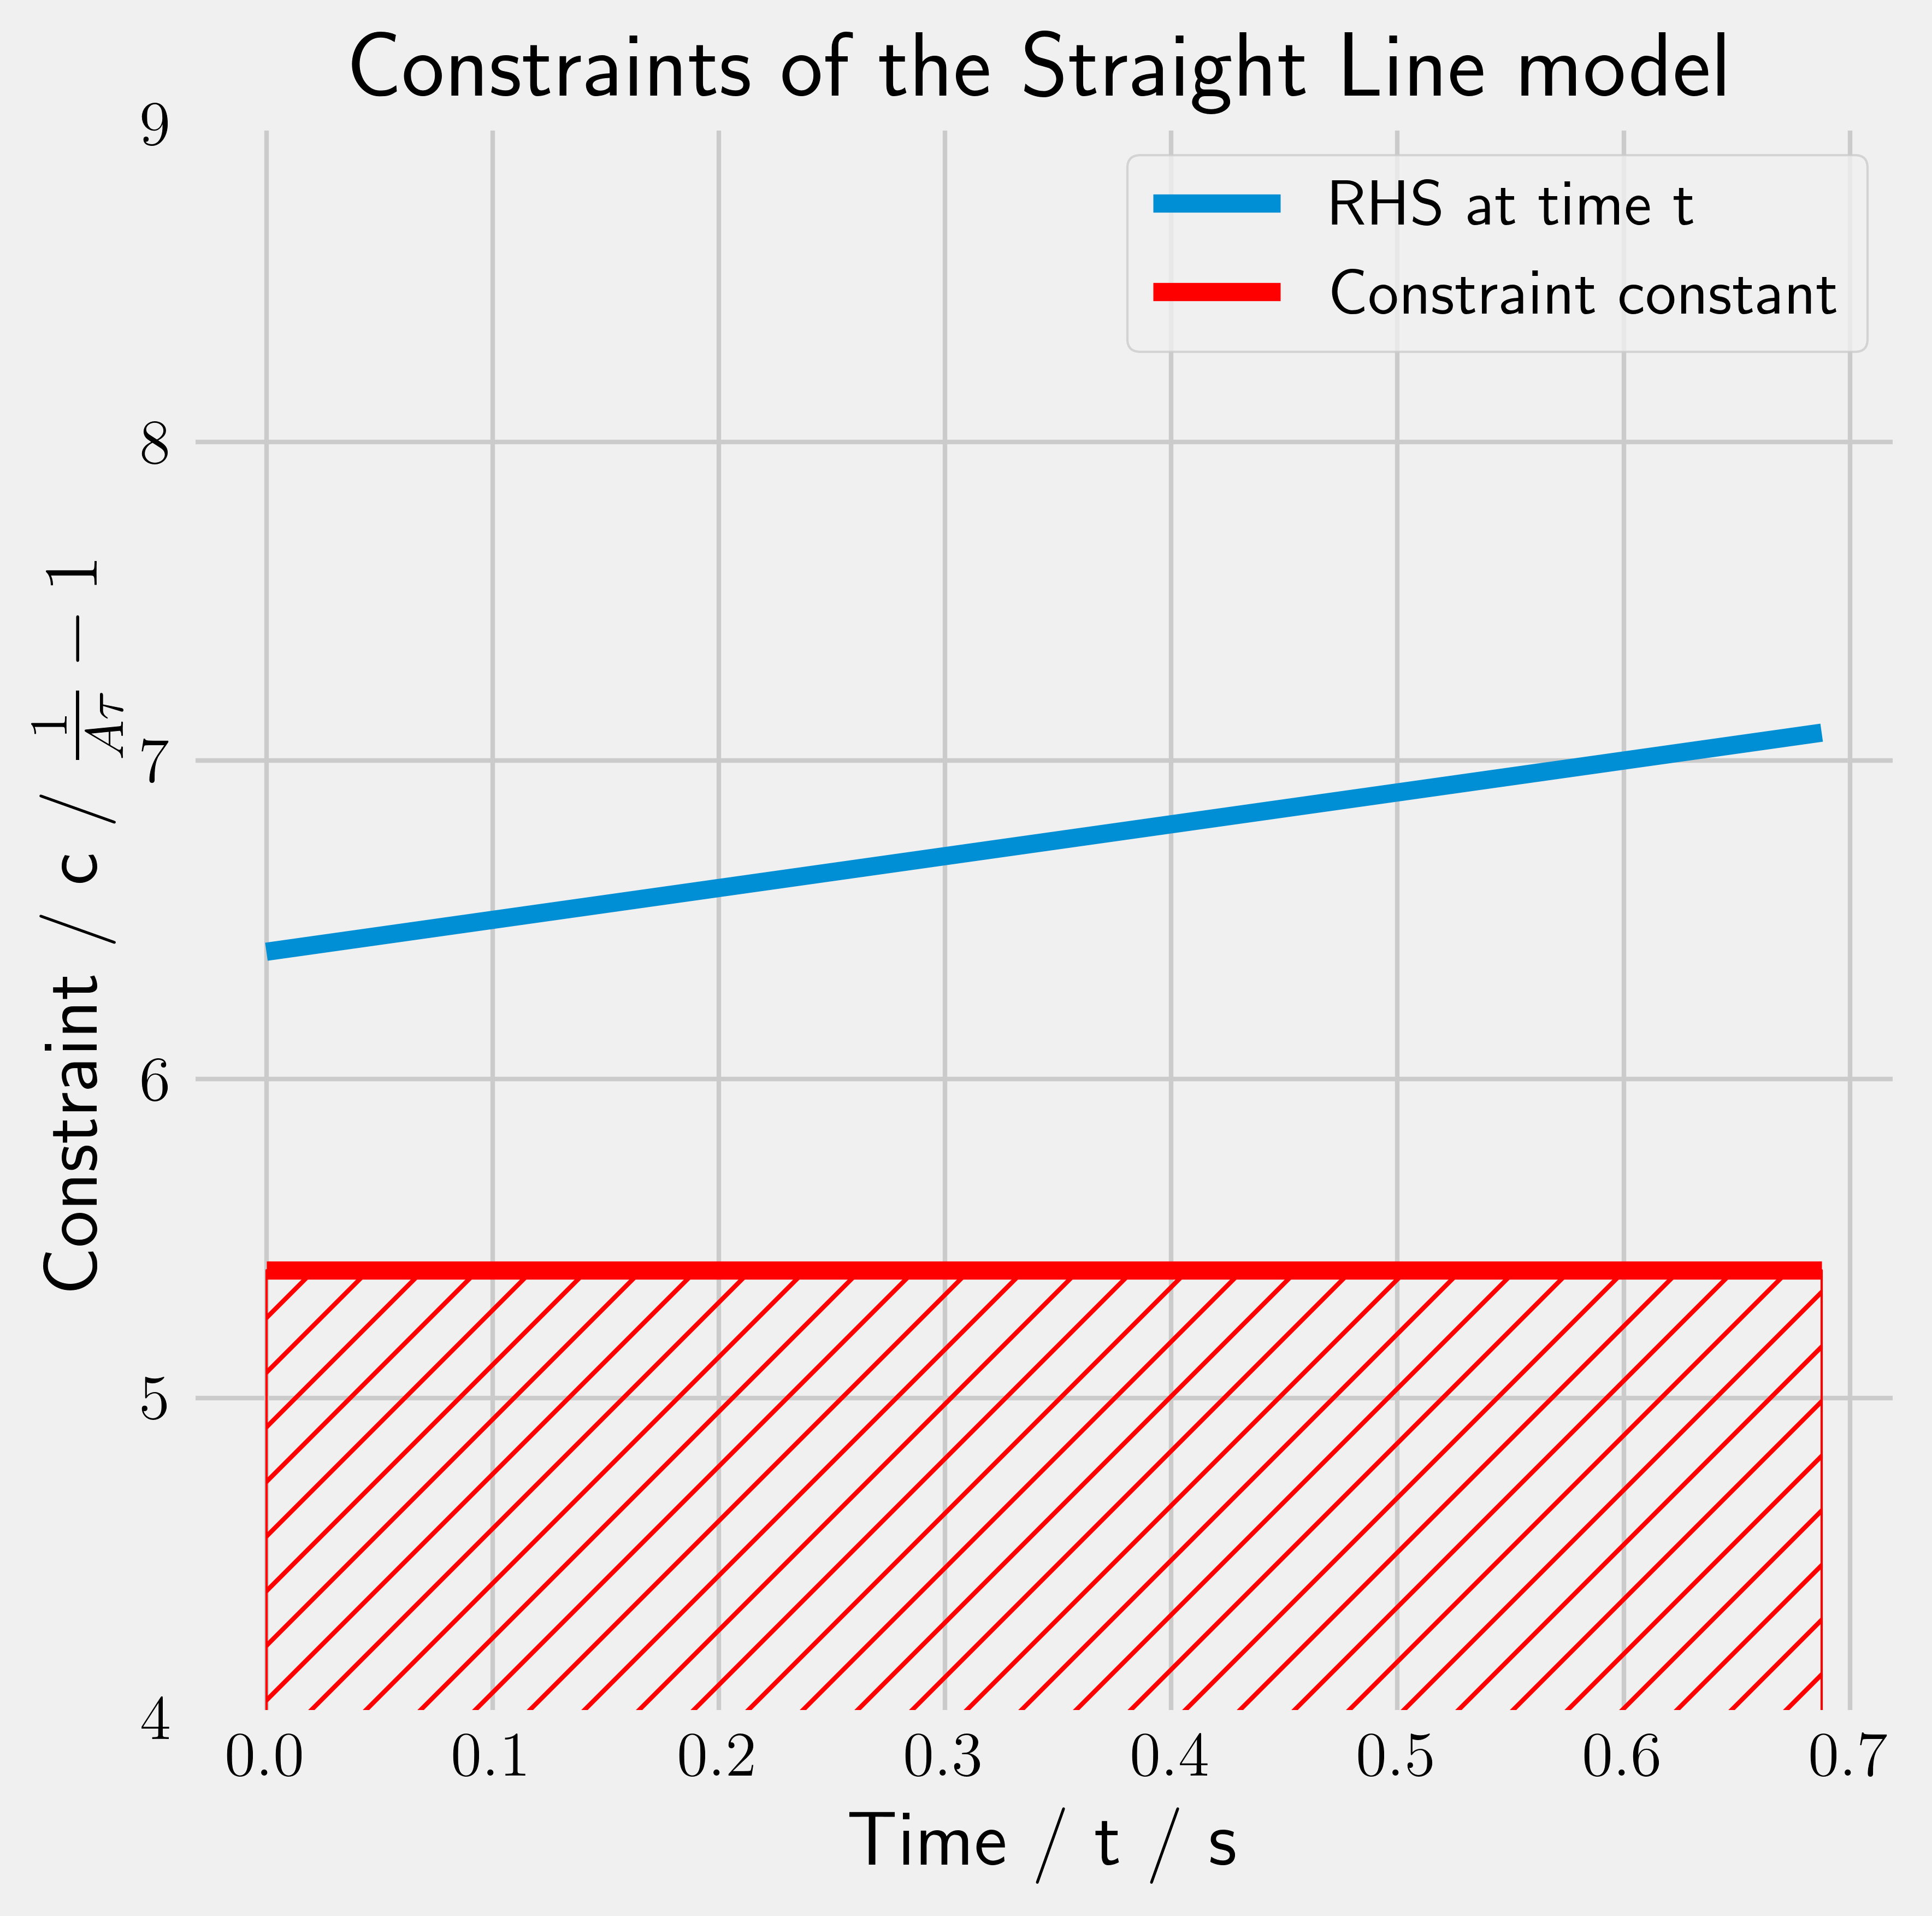
\includegraphics[width=0.45\textwidth,right]{assets/straight_constraint_inequality.png}
    \caption{}
    \label{fig:straight_constraint_inequality}
\end{wrapfigure}

But the game analyzed does have the constraint of a speed limit so players cannot accelerate infinitely, traveling across the map in two-to-three seconds. The graphing of the constraint (equation \ref{eq:constraint}) shows the problems (figure \ref{fig:straight_constraint_inequality}).

It is obvious that the RHS (top line) is higher than the constraint LHS (bottom shaded area). This indicates that the player exceeds the speed limit for every time within the considered time domain, which will undoubtedly massively decrease the restricted displacement. The inequality of the RHS can be represented symbolically by substitution of the player acceleration function into equation \ref{eq:constraint}:
\[
    5.4 \ge t + \frac{v_{0y}}{w}.
\]

Because the variable $\frac{v_{0y}}{w} = 6.4$, the inequality will only hold in negative $t$, which is not in the time domain considered. Only when the initial y-axis velocity is below $\frac{5.4 w}{v_{0y}}$ would there be acceleration on the first frame.

Therefore the restricted player motion would be without any acceleration at any time. The continuous displacement of the player at time $t_f$ can be computed by setting the variable $w=0$, or:
\begin{align*}
 \tp(t)_x &= t v_{0x} = 0\\
 \tp(t)_y &= t v_{0y}\\
 \tp(t_f)_y &= 0.7 \times 250 = 175.
\end{align*}

The discrete restricted jumping equation using Euler's method (figure \ref{eq:rje}) resulted in a similar distance of $175.78$, using constant $h=\tau$. Furthermore I've noticed that the displacement/time graph (figure \ref{fig:straight_constraint}) have displacements equality spaced in the y-axis --- in contrast with the ever expanding dots in the unrestricted case (figure \ref{fig:straight_nothing_1}). I believe that this indicates a lack of acceleration, which greatly reduced the result of this baseline model. Furthermore, the lack of acceleration means that this model can also be achieved with no player inputs, as the minimum value of acceleration $w$ is zero.

\begin{wrapfigure}{r}{0.48\textwidth}
    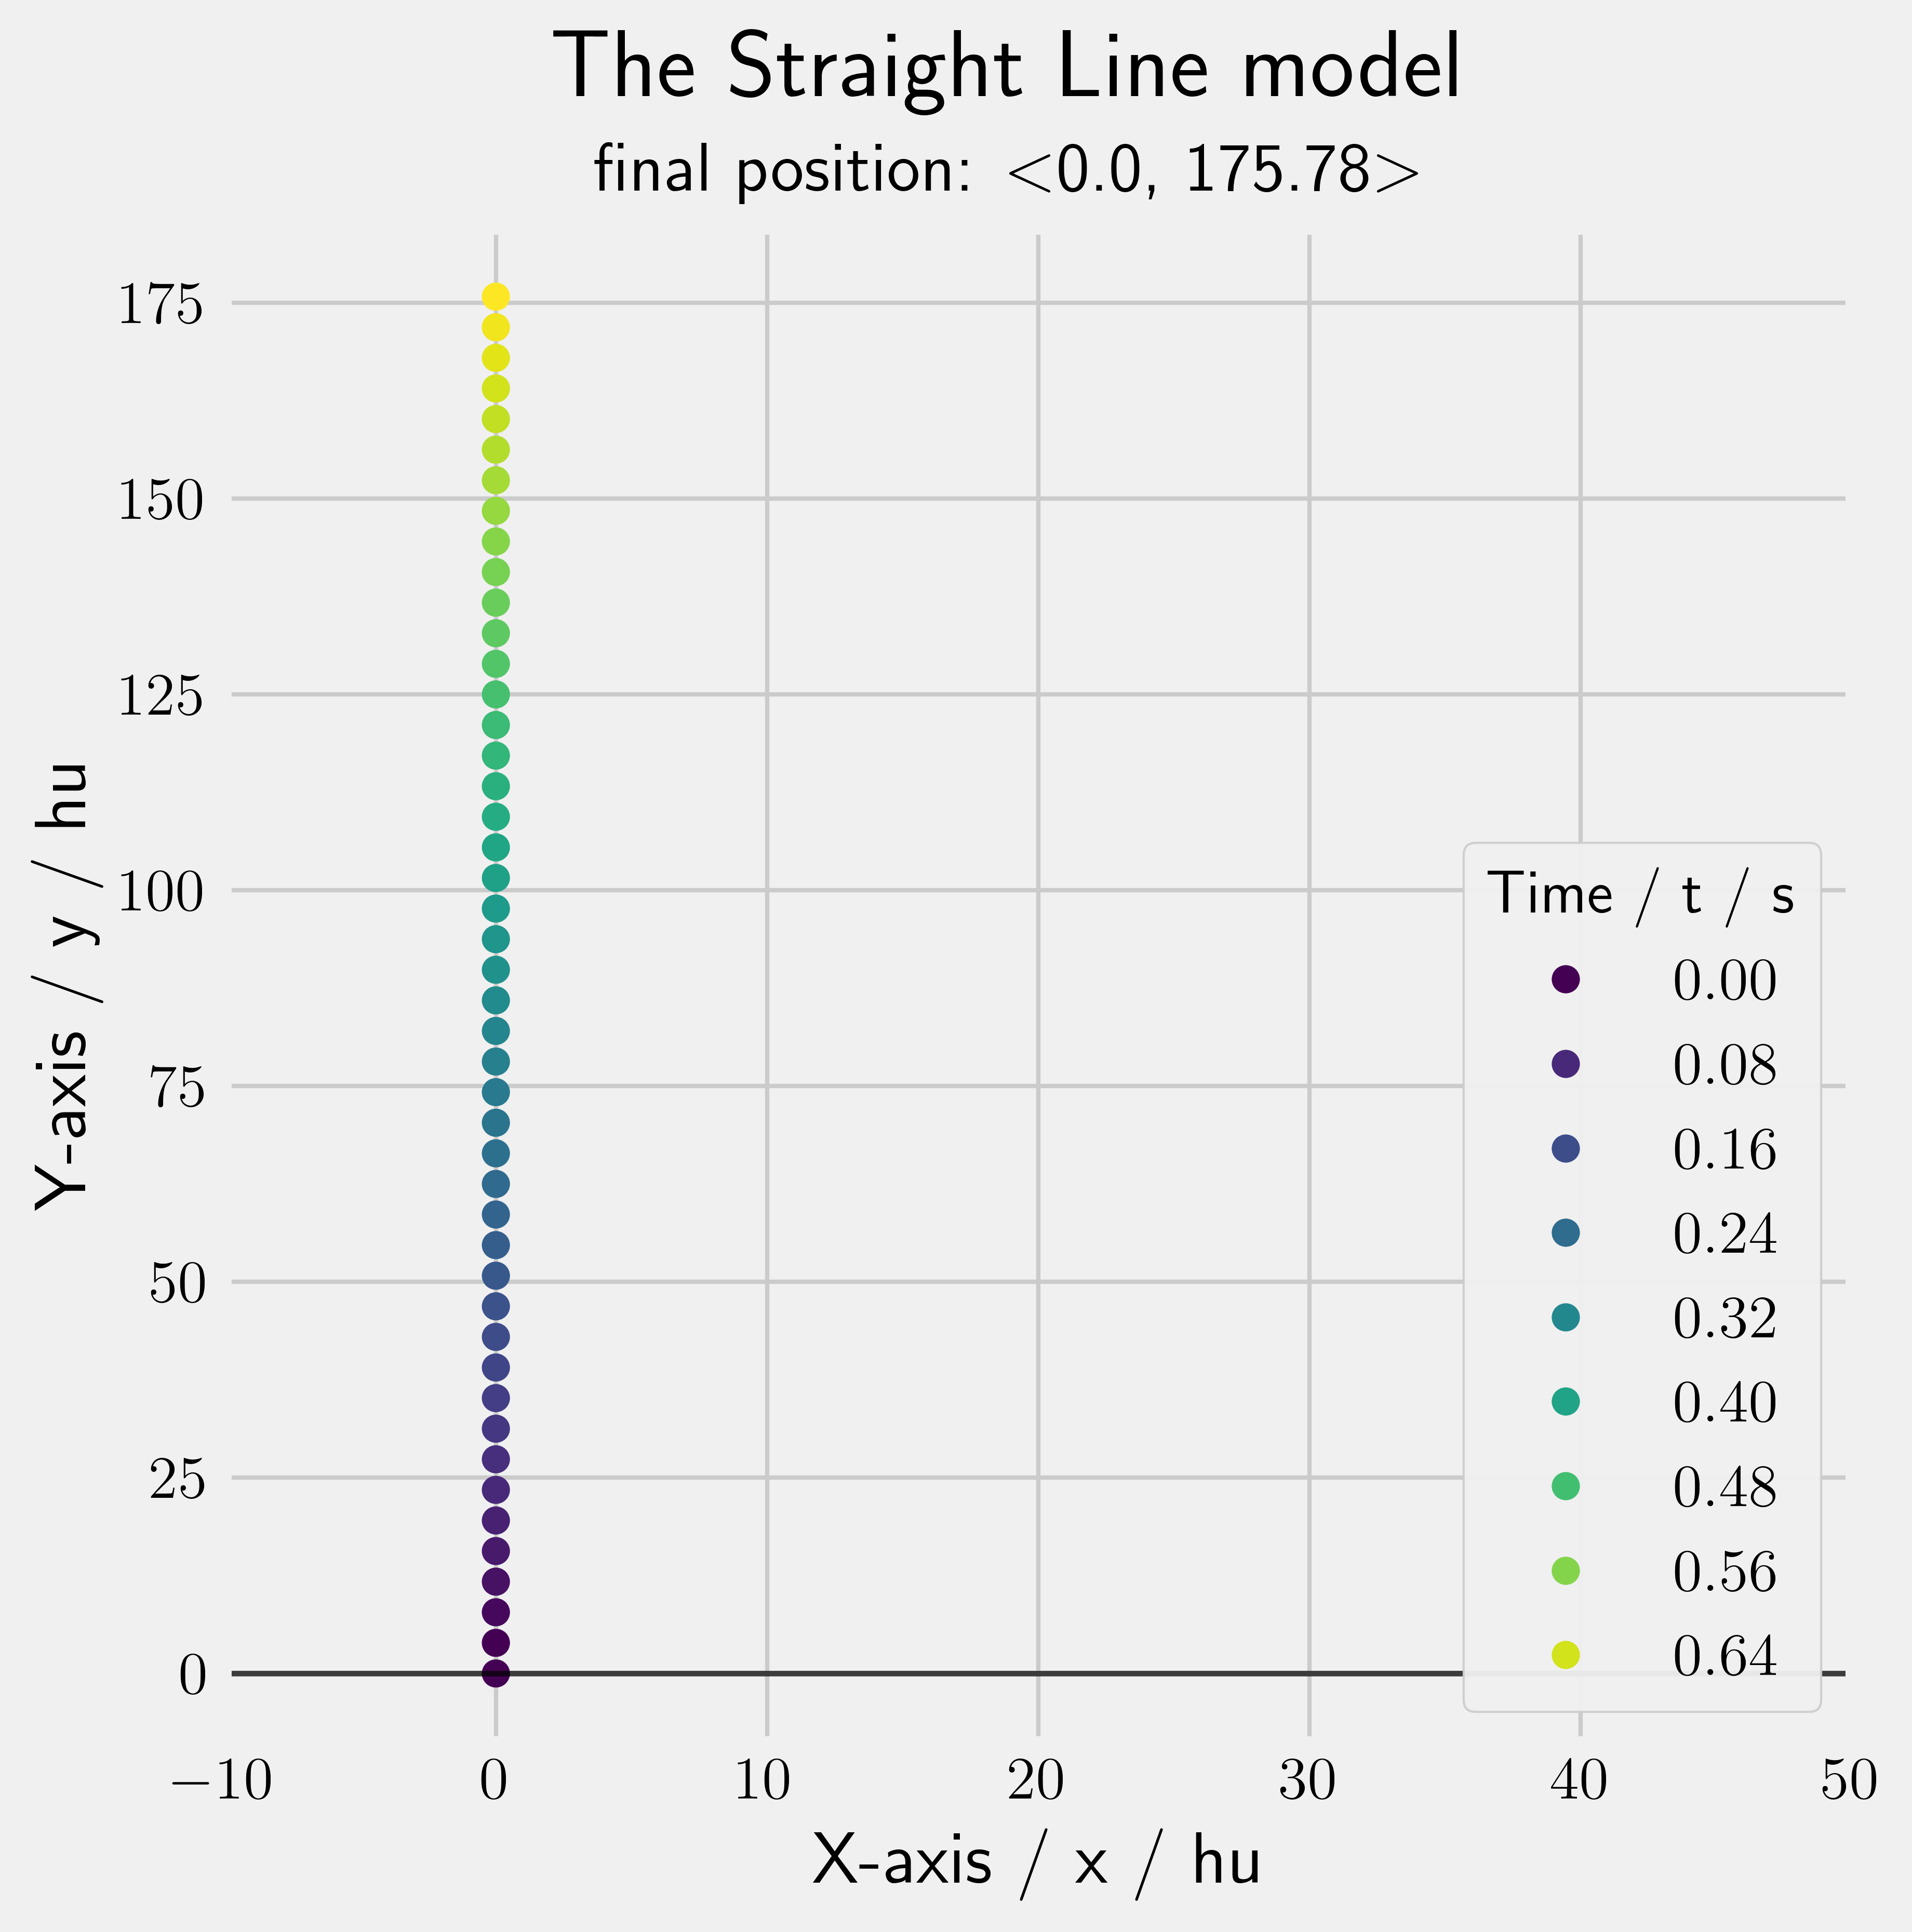
\includegraphics[width=0.45\textwidth,right]{assets/straight_constraint.png}
    \caption{}
    \label{fig:straight_constraint}
\end{wrapfigure}

Overall, the straight-line model establishes the baseline of my analysis. Using this strategy, the player has traveled an average distance in a jump of around $175$ hammerunits, which is well below what I can achieve in-game. The method has the benefit of requiring no input from the player, and can be performed consistently every  time. This makes the method the best model to conserve human energy by minimizing the amount of effort. But we can do better.

% conclusion

% Do not have enough words for this machine learning step
%\subsection{Machine learning}
%To kick start the optimization step, I decided to utilize the computing power I have access to to run a machine learning model on this problem. The result of which can potentially be graphed and fitted a model against, which could potentially be optimized further.

%From my previous experience in strafing sub-optimally, I hypothesize that

% state the steps of this

\subsection{Step by step}
My second model would be trying to optimize the y-axis displacement with each discrete change in time. Reflect back to subsection where I defined the restrictions (\ref{eq:constraint}), where the movement integrated vector functions must satisfy an inequality for maximum acceleration. This is problematic for this method in that the integrated player acceleration function $X(t)$ and $Y(t)$ have no obvious relationships, as it does not need to be a vector with unit length 1. I tried to define $x(t)$ in terms of $y(t)$ with
\[
    x(t) = \sqrt{1-y(t)^2},
\]
but found the integral
\[
    X(t) = \int \sqrt{1-y(t)^2} \, dt
\]
a pain or sometimes impossible to solve analytically. I needed to represent acceleration in another form preferably in a single variable function --- I attempted to do it with polar coordinates.



%I found the constraint equations to be difficult to use because it contains two related functions as input: $X(t)$ and $Y(t)$. This is because the solution to the problem is currently of form $x(t)$, which is the x component of acceleration as a function of time. Therefore the first integral $Y(t)$ must be in the form:
%\[
%    Y(t) = \int \sqrt{1-x(t)^2} \, dt,
%\]
%which turns out to be a very difficult integral to solve analytically. Therefore I attempted to derive the equations of motions again in polar coordinates, because I realized that I can represent player acceleration with a single function $\theta(t)$, which removes the square root function in the constraint inequality and allowing optimizations frame by frame.

% TODO: Finish writing this

\subsubsection{Equations of motion, angular}
Let the player displacement $\tp$, velocity $\tv$ be complex numbers with the real part the x-axis and the imaginary part the y-axis. They are represented in the Euler forms (where the function $\exp(x)= e^{x}$ for simplicity):
\begin{align*}
    \tp &= a \exp(b \I)\\
    \tv &= r \exp(\phi \I),
\end{align*}
where $a$ and $r$ are the magnitudes of the player displacement and velocity, and $b$ and $\phi$ are their respective angles from the x-axis.

Define the player acceleration in terms of the smallest angle between the unit vector $\tunit{a}$ and the velocity $\tv$, denoted as $\theta(t)$ as a function of time (figure \ref{fig:angular}).

\begin{wrapfigure}{r}{0.40\textwidth}
    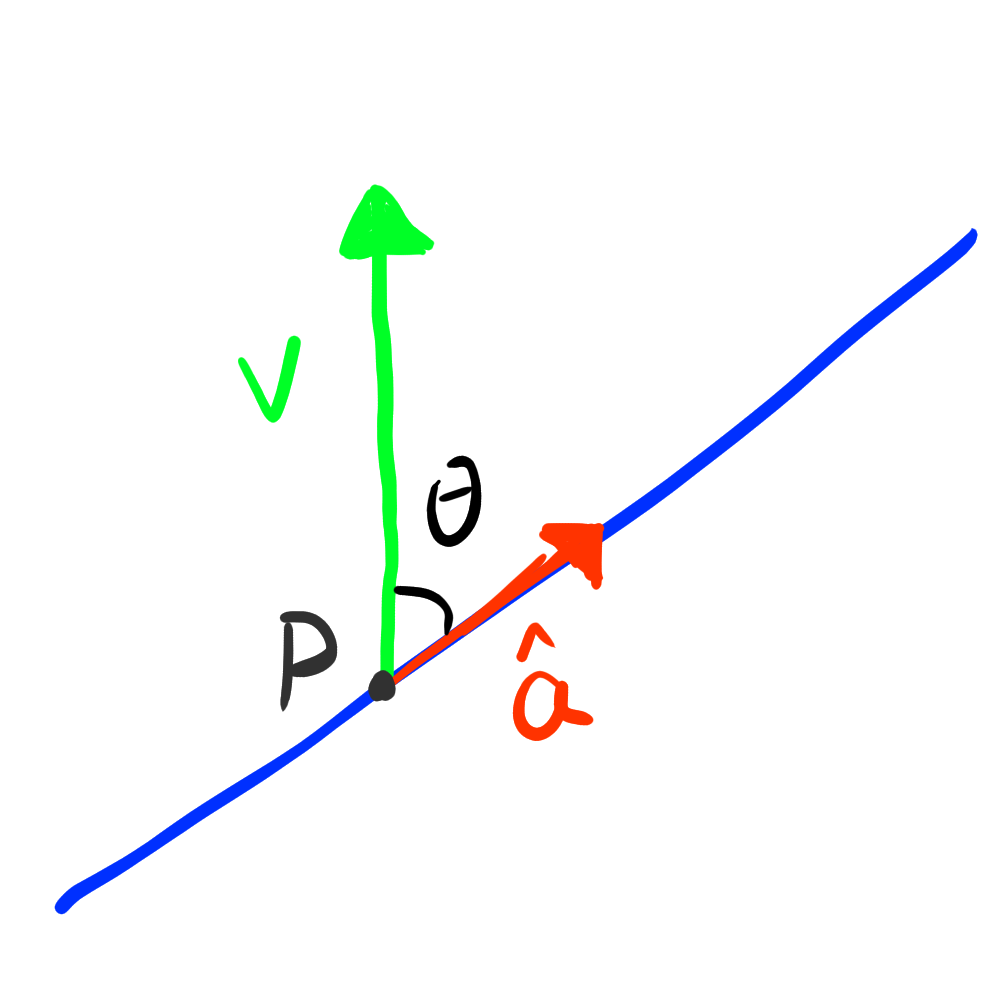
\includegraphics[width=0.37\textwidth,right]{assets/angular.png}
    \caption{The angular function}
    \label{fig:angular}
\end{wrapfigure}

Notice that the angular function $\theta(t)$ is the angle between the acceleration unit vector and the velocity vector, so it has a unit length with angle $\phi - \theta$:
\[
    \tunit{a} = \exp((\phi - \theta) \I).
\]

We can then rewrite the discrete velocity update at each timestep $\tau$ as so:
\begin{align*}
    \tv' &= \tv + w \tunit{a}\\
    \tv' &= \tv + w \exp((\phi - \theta) \I),
\end{align*}
where $w$ is the piecewise function in step 3. Also, the position update is unchanged:
\[
    \tp' = \tp + \tau \tv.
\]

In order to maximize jumping displacement, it seems reasonable to maximize velocity and therefore maximize acceleration. This means to maximize the scalar $w$, which is equivalent to finding a function that fits the constraint in equation \ref{eq:constraint}.

Remember that the scalar function $w$ is defined piecewise:
\[
    w = \begin{cases}
        \gamma_1 & \gamma_2 \ge \gamma_1\\
     \gamma_2 & \gamma_1 > \gamma_2 > 0\\
     0 & 0 \ge \gamma_2
    \end{cases},
\]
where $\gamma_1 = LA\tau$ and $\gamma_2 = L - \tv \cdot \tunit{a}$. This can be rewritten in terms of our new angular function $\theta(t)$.

Consider the case of maximum acceleration, where $w=\gamma_1$. The inequality condition can be rewritten as:
\begin{align*}
    \gamma_2 &\ge \gamma_1\\
    L - \tv \cdot \tunit{a} &\ge LA\tau\\
    L - \tmag{v} \cos \theta &\ge LA \tau\\
    L - LA\tau &\ge \tmag{v} \cos \theta\\
    \frac{L - LA\tau}{\tmag{v}} &\ge \cos \theta\\
    \cos^{-1} \frac{L - LA\tau}{\tmag{v}} &\ge \theta.
\end{align*}
This shows that $\theta(t)$ must be greater or equal to a LHS function for maximum acceleration to happen.

Now consider the case of minimum acceleration, where $w=0$. The inequality condition is:
\begin{align*}
    \gamma_2 &\le 0\\
    L - \tv \cdot \tunit{a} &\le 0\\
    L &\le \tmag{v} \cos \theta\\
    \frac{L}{\tmag{v}} &\le \cos \theta\\
    \cos^{-1}  \frac{L}{\tmag{v}} &\le \theta.
\end{align*}
This shows that $\theta(t)$ needs to be smaller than a function for minimum acceleration to happen.

Therefore, we can rewrite the piecewise function $w$ with:
\[
w = \begin{cases}
    \gamma_1 & \cos^{-1} \frac{L - LA\tau}{\tmag{v}} \ge \theta\\
    \gamma_2 & \text{otherwise}\\
    0 & \cos^{-1}  \frac{L}{\tmag{v}} \le \theta
\end{cases}.
\]

\subsection{Optimization}
Using the same argument as the straight-line model, I will use an initial velocity of $\tv_0 = \tang{0, 250}$.

Firstly notice that for maximum acceleration magnitude, the player want to minimize $\theta(t)$. This is due to the the law of cosine (\ref{fig:min_theta}).

\begin{wrapfigure}{r}{0.40\textwidth}
    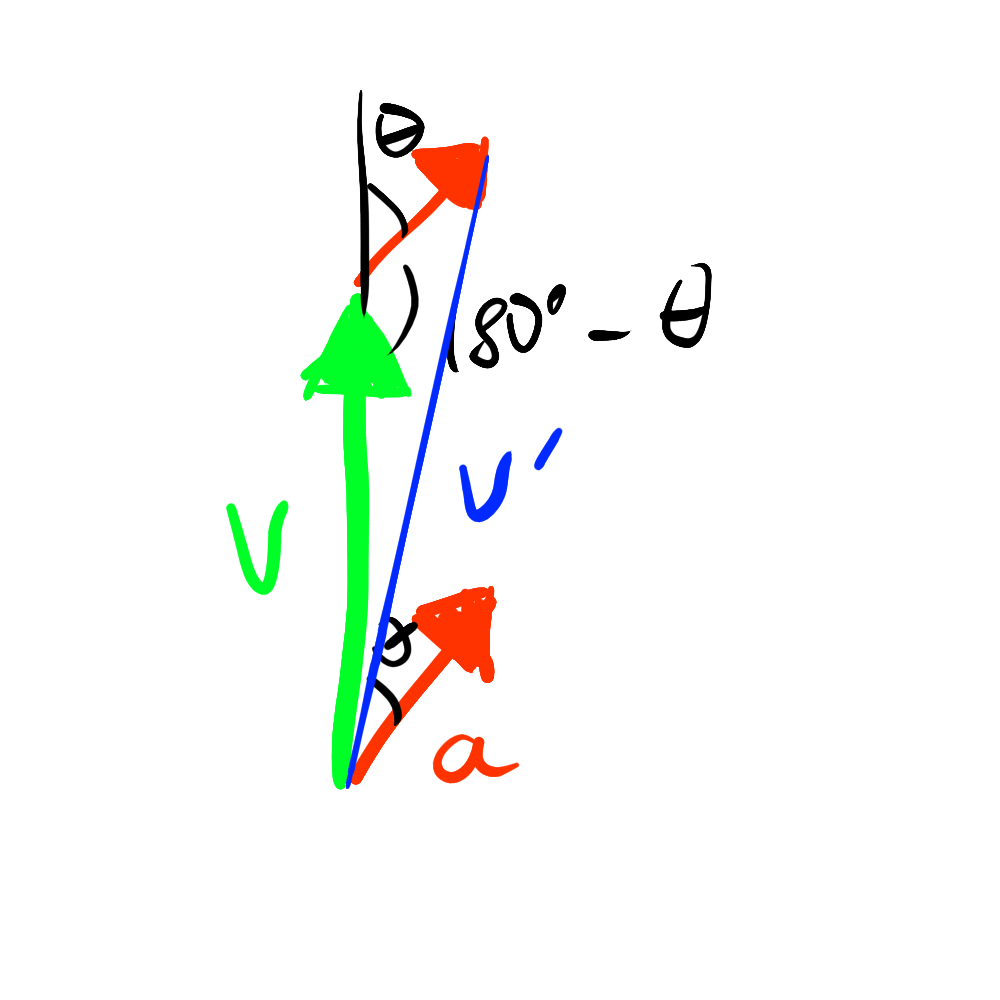
\includegraphics[width=0.37\textwidth,right]{assets/min_theta.png}
    \caption{Minimizing $\theta(t)$}
    \label{fig:min_theta}
\end{wrapfigure}

Let $v = \tmag{\tv}$, $a = \tunit{a}$. The length of the hypotenuse
\[
    v' = \sqrt{v^2 + a^2 -2 va \cos (\pi - \theta)}
\]
is the magnitude of the updated velocity. To maximize $v'$ means minimizing $\cos(\pi - \theta)$, as $v$ and $a$ are constant per timeframe. For the cosine function is smaller at higher x values, we need to maximize $\pi - \theta$ and therefore minimize $\theta$.

Thus for maximum acceleration, the player needs to minimize $\theta$ while keeping $\theta$ above a value at every time frame. I believe we can optimize the player displacement by setting $\theta$ to equal the value at all times, and that:
\[
    \theta = \cos^{-1} \frac{L-LA\tau}{\tmag{v}}.
\]

Notice that the $\theta$ increases as the magnitude of velocity increases, showing that acceleration must decrease as velocity increases. Additionally, the maximization of velocity at every step does not necessarily maximize the player displacement --- a very high velocity pointing towards the origin of jump is more harmful than good.

By substituting this equation of $\theta$, I derived the first step by step difference equation:
\begin{figure}[H]
    \centering
    \[
        d\tv = LA\tau \exp((\phi - \cos^{-1}(\frac{L-LA\tau}{\tmag{v}})) \I).
    \]
    \caption{First Step by Step difference equation}
    \label{fig:sbs}
\end{figure}

Figure \ref{fig:1sbs} shows the player's motion under this method.
\begin{figure}[H]
    \centering
    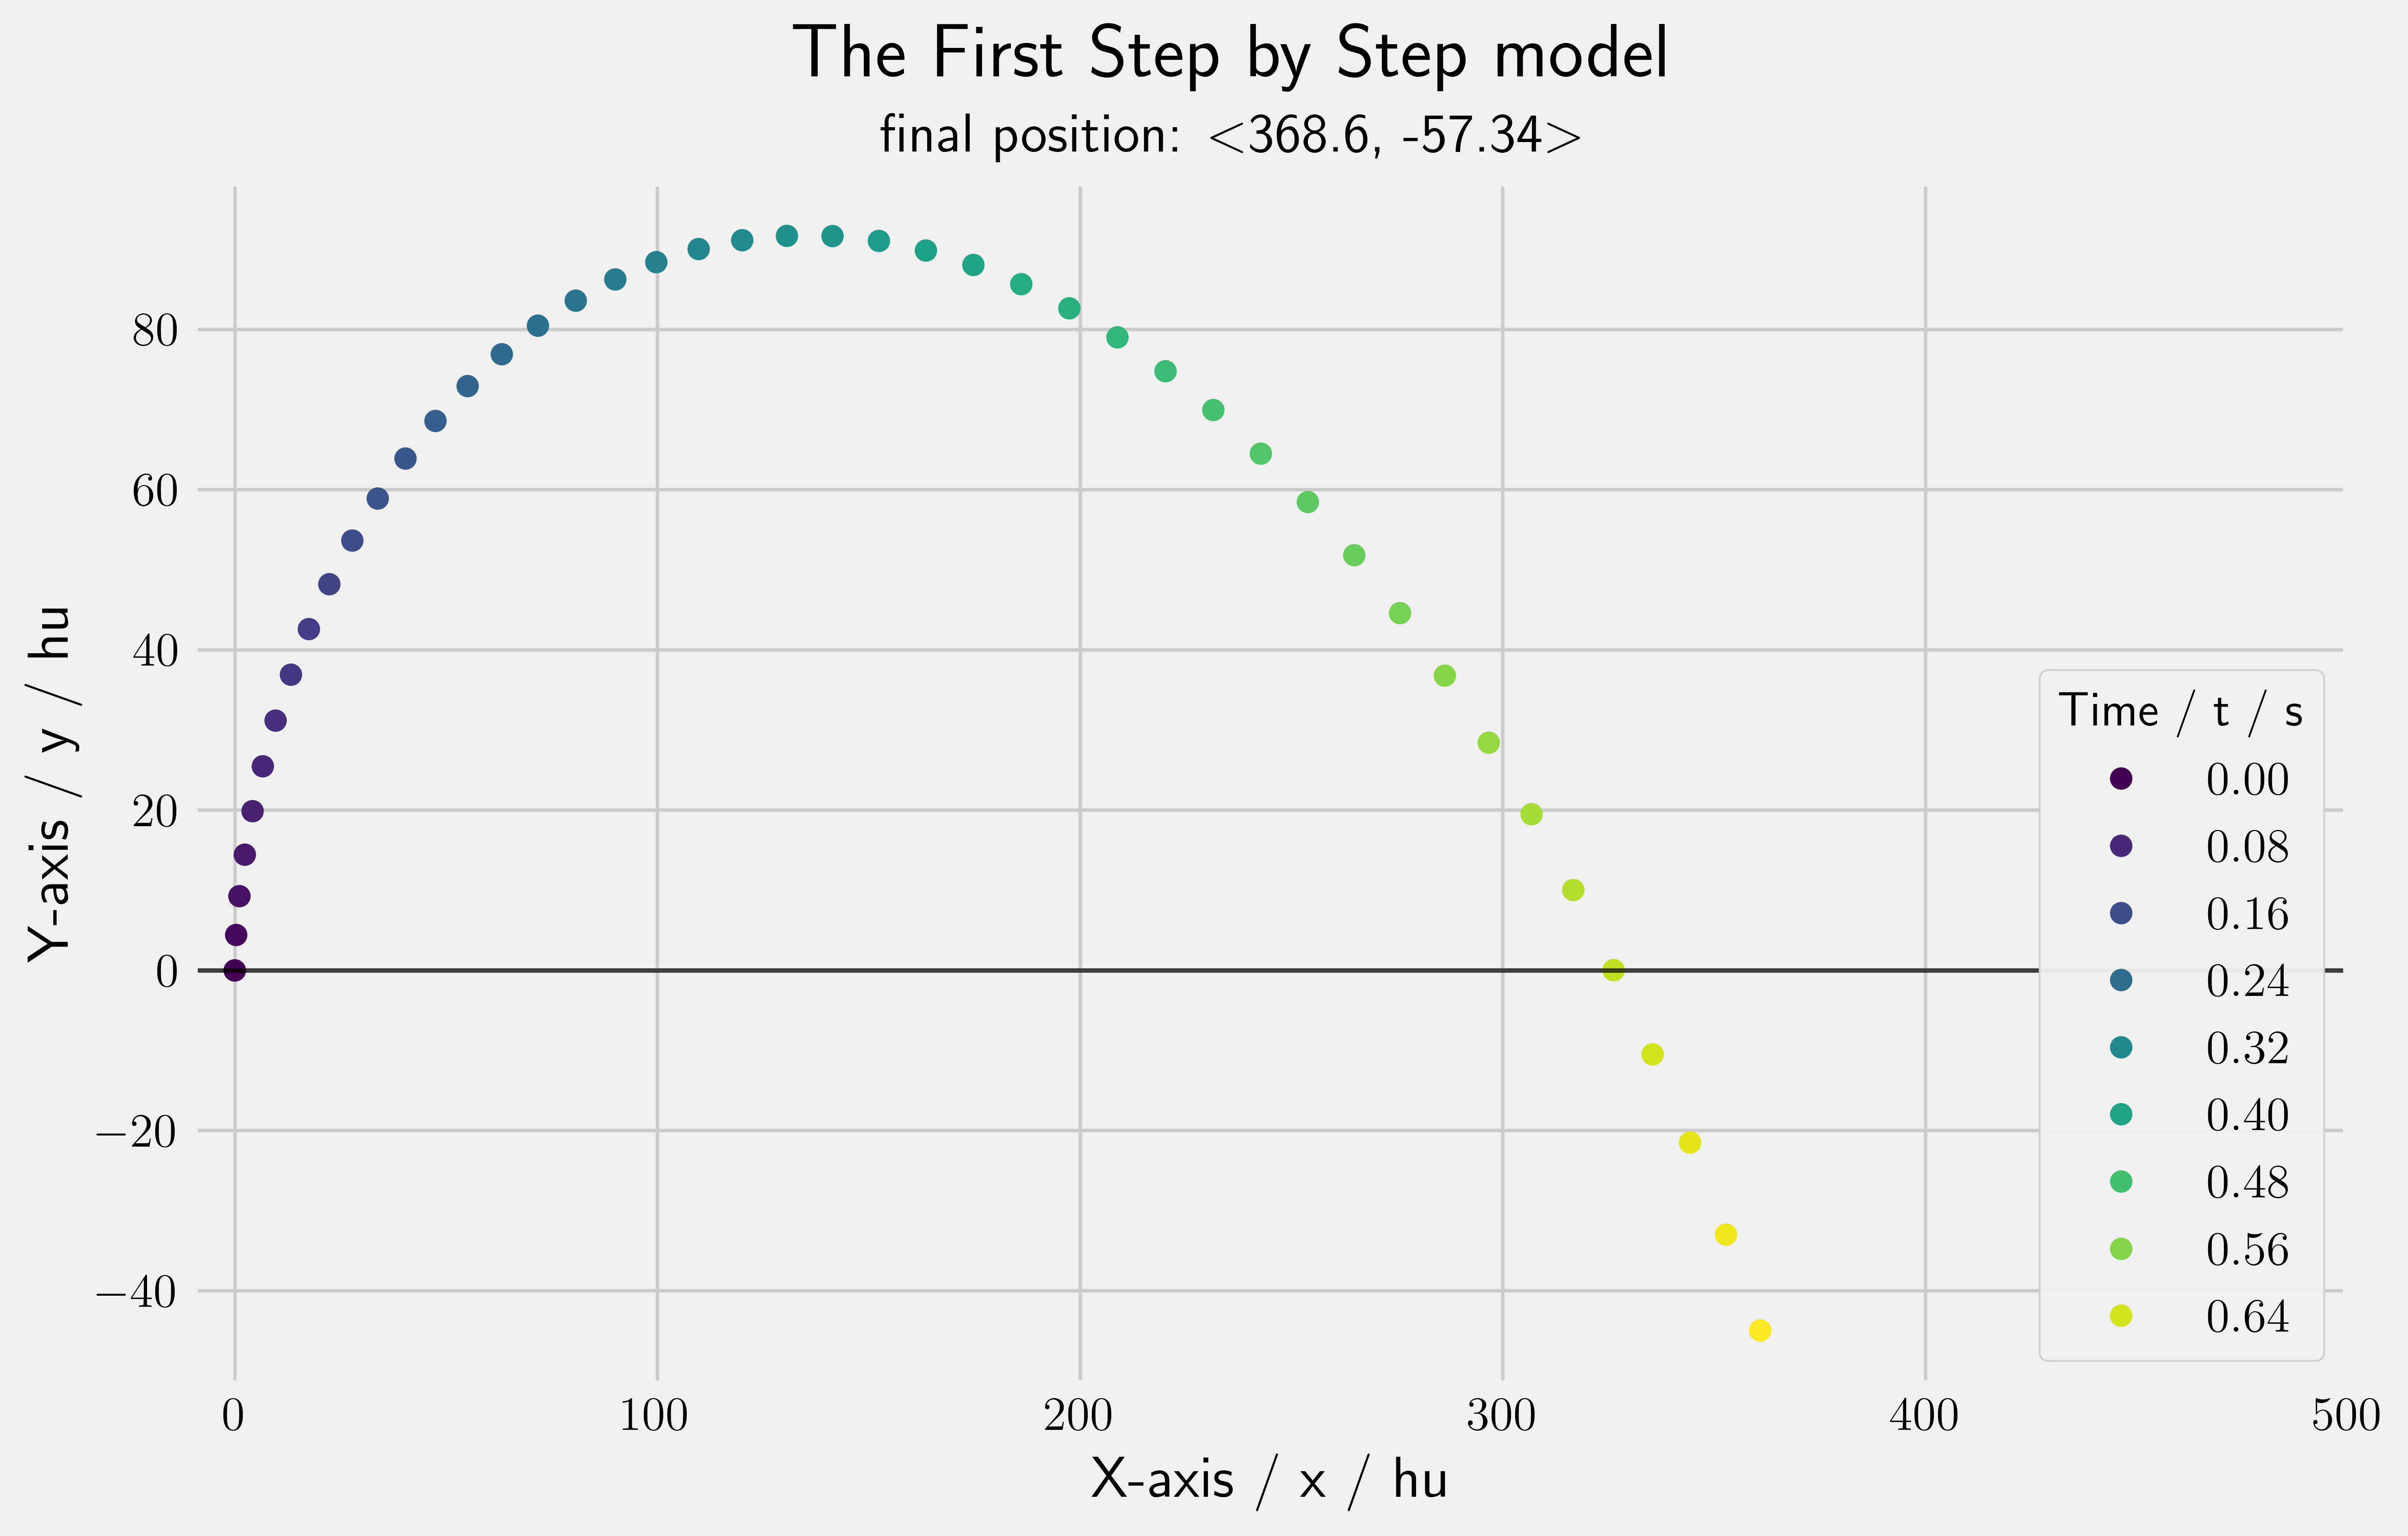
\includegraphics[width=0.8\textwidth]{assets/step_by_step_1.png}
    \caption{}
    \label{fig:1sbs}
\end{figure}

Oops, it looks like we've done a u-turn and ended up below the x-axis. Although the spacing between each timeframe dots are increasing --- indicating acceleration, the method had to keep turning for maximizing velocity which potentially reduced our displacement. Nevertheless, this first method had a displacement of $\sqrt{368.6^2 + (-57.34)^2} \approx 373.0$, which is a large increase from the straight-line model's $175$ units.

\subsection{Step by Step with modification}
The first step by step model (figure \ref{fig:1sbs}) had a problem, that the player needed to turn more than $90$ degrees to keep accelerating. This sounds counter-intuitive, so I have two ideas to fix it: stop turning at a specific angle or accelerate below the maximum value.

The arguments for stop turning at a specific angle is that we are sacrificing higher velocity and less distance traveled but preferring more forward movements, which could potentially increase the total displacement. I decided to set a maximum angle for player velocity, which once reached, would











\subsection{Euler-Lagrange optimization}


% TODO: calculated the restricted line,

% TODO: conclude this: max 250 total words

% TODO Have around 1500 words

% 500 words each for each method

% 500 for conclusion

Do the step by step one

Do the euler-lagrange one

Extension, find the optimal angle for each

